\documentclass[11pt]{article}

\usepackage[a4paper,margin=2.4cm]{geometry}
\usepackage{amsmath,amssymb}
\usepackage{booktabs}
\usepackage{siunitx}
\usepackage{graphicx}
\usepackage{xcolor}
\usepackage[hidelinks]{hyperref}
\usepackage{enumitem}

\newcommand{\bplus}{\beta^{+}}
\newcommand{\Cl}[1]{{}^{#1}\mathrm{C}}
\newcommand{\Ox}[1]{{}^{#1}\mathrm{O}}
\newcommand{\Nt}[1]{{}^{#1}\mathrm{N}}
\newcommand{\Rd}{R_{\mathrm d}}
\newcommand{\Rp}{R_{\mathrm p}}
\newcommand{\tirr}{t_{\mathrm{irr}}}
\newcommand{\tdel}{t_{\mathrm{del}}}
\newcommand{\tmeas}{t_{\mathrm{meas}}}

\title{Proton-therapy PET range verification:\\
the physics of the positron-emitter source}
\author{J.J. G\'omez-Cadenas\\\texttt{jjgomezcadenas@gmail.com}}
\date{Documentation last rebuild: \today}

\begin{document}
\maketitle

\begin{abstract}
Proton therapy concentrates dose at the Bragg peak, which makes the proton range
the quantity to verify. The verification signal is the positron emitters created
along the beam by nuclear fragmentation, imaged by PET. This note collects the
physics behind that signal: how the induced $\bplus$ activity arises and decays in
time, how the measured number of decays follows from the production through
radioactive decay and the acquisition timing, how the activity distribution
relates to the dose, and how a spread-out Bragg peak field that paints a uniform
dose over a target is built --- analytically for a homogeneous phantom, and in
water-equivalent path length for a heterogeneous head. The operational side, how
the simulation is run and how the resulting source is used, is in the companion
user guide.
\end{abstract}

\section{Tracking proton dose with \texorpdfstring{$\bplus$}{beta+}}
\label{sec:physics-intro}

Conventional, photon-based radiation therapy deposits a high dose where the beam enters the patient, weakening gradually as it traverses tissue. A proton beam instead releases most of its energy near the end of its track, at the so-called Bragg peak; combining protons of several energies produces a spread-out Bragg peak (SOBP). The proton entrance dose is therefore much lower and no dose is deposited beyond the target volume. This lets proton therapy shape the high-dose region to the three-dimensional outline of the target while sparing the surrounding tissue, making it preferable for tumours with irregular shapes or close to critical structures. Its integral dose is also much smaller, about 60\% below that of photon therapy, which favours its use in paediatric patients, where the risk of a secondary tumour induced by dose to normal tissue is a concern~\cite{parodi2023, parodi2024}.

The steep dose fall-off at the Bragg peak makes planning uncertainties more consequential than in photon therapy. A range error can leave part of a tumour with no dose at all (under-shooting), or deliver a full dose to the normal tissue lying distal to the beam (over-shooting). Verification is therefore of utmost importance, both to exploit the technique and to assess treatment-planning safety margins. Since proton beams stop completely in the body, direct in vivo monitoring is difficult, and at present the only practical approach is PET imaging of the proton-induced positron emitters.

During irradiation, positron emitters are produced along the beam path through nuclear fragmentation, leaving a radiotracer footprint that a PET scanner can image. In soft tissue the main species are $\Cl{11}$, $\Nt{13}$ and $\Ox{15}$. The last dominates right after irradiation, owing to the high oxygen density of tissue, but its short half-life (about 2 minutes) means $\Cl{11}$ takes over after a few minutes~\cite{zhu2013proton}.

Dose deposition and positron-emitter production are distinct processes: dose is deposited electromagnetically, by ionising and exciting atomic electrons, whereas emitter production proceeds through nuclear reactions whose yield depends on proton fluence, energy-dependent reaction cross sections and target-nuclei density. The PET activity distribution is thus quite different from the dose distribution, with almost no activity in the $\sim$1~cm before the Bragg peak, owing to nuclear reaction thresholds; the measured activity must therefore be compared with a predicted distribution.

\subsection{Induced activity and its time evolution}
\label{sec:activity}

Protons traversing biological tissue undergo nuclear reactions, such as for example,
$p + \Ox{16} \rightarrow \Ox{15} + n + p$, followed by
$\Ox{15} \rightarrow \Nt{15} + \bplus + \nu_e$ ($T_{1/2} = 122\,\mathrm{s} \approx\SI{2}{min}$).
Other relevant $\bplus$ emitters are $\Cl{11}$ ($T_{1/2}\approx\SI{20}{min}$), $\Nt{13}$ ($T_{1/2}\approx\SI{10}{min}$),
and the shorter-lived $\Ox{14}$ ($T_{1/2}=\SI{70.6}{s}$) and $\Cl{10}$
($T_{1/2}=\SI{19.3}{s}$)~\cite{zhu2013proton,parodi2008comparison}. Because the
signal is a mixture of species with very different half-lives, the measurement
depends strongly on when the scanner acquires.

\begin{figure}[htbp]
\centering
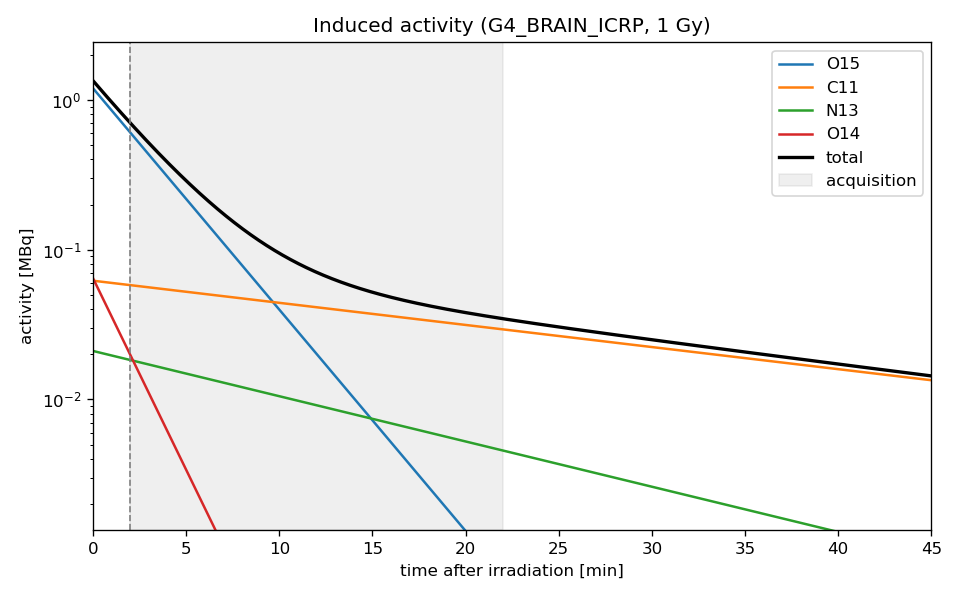
\includegraphics[width=0.8\linewidth]{activity.png}
\caption{Activity of the main positron-emitting species as a function of time after
irradiation, from a Geant4 simulation of a \SI{1}{Gy} proton field in an ICRP
brain-tissue phantom. The shaded band marks a representative in-room acquisition
window. The shortest-lived emitter, $\Cl{10}$ ($T_{1/2}=\SI{19.3}{s}$), has
effectively vanished before the window opens and is not drawn.}
\label{fig:activity}
\end{figure}

Figure~\ref{fig:activity} shows the activity by species from a Geant4 simulation of
a \SI{1}{Gy} proton field in an ICRP brain-tissue phantom.
The total peaks at $\sim$\SI{1.34}{MBq} at the end of the beam, dominated by
$\Ox{15}$ at $\sim$\SI{1.2}{MBq}. But $\Ox{15}$ decays with a \SI{2}{min} half-life:
by \SI{10}{min} it has fallen to the level of $\Cl{11}$, and by $\sim$\SI{15}{min}
it has effectively gone. The very short-lived emitters disappear even sooner ---
$\Cl{10}$ within about a minute, $\Ox{14}$ within a few. The $\Cl{11}$ component is
nearly flat ($T_{1/2}\approx\SI{20}{min}$) at $\sim$\SI{0.06}{MBq} and comes to
dominate after $\sim$\SIrange{10}{13}{min}.

Two consequences follow from this decay pattern. First, the scan must start as soon as possible after the beam stops, since an in-beam scan can be impractical because of backgrounds. Second, every photon pair is precious. These two requirements are somewhat contradictory. An immediate scan requires an in-line PET, which must let the beam through; the resulting open geometry has poor geometrical acceptance. The opposite approach, moving the patient to an off-room PET, is also impractical: after about five minutes the activity has fallen sharply, through both isotope decay and biological washout. An in-room PET --- a full-ring scanner in the treatment room --- is an affordable compromise. An in-room scan at $\sim$\SI{2}{min} still sees $\sim$\SI{0.7}{MBq}, with $\Ox{15}$ still dominant; an offline scan at $\geq$\SI{15}{min} sees only $\sim$\SI{0.04}{MBq}, essentially $\Cl{11}$ alone --- more than an order of magnitude less signal.

\section{Decay kinetics: from produced emitters to measured decays}
\label{sec:kinetics}

Each species $j$ decays with constant $\lambda_j=\ln 2/T_{1/2,j}$ and is taken to
decay $100\%$ by $\bplus$. Consider a delivery of duration $\tirr$ at an
approximately constant production rate $K_j=P_j/\tirr$, where $P_j$ is the integral
production of species $j$ over the whole field. Production and decay proceed
together during the beam and decay alone afterwards, so the activity is
\begin{align}
A_j(t) &= K_j\bigl(1-e^{-\lambda_j t}\bigr), & 0\le t\le \tirr,\\
A_j(t) &= K_j\bigl(1-e^{-\lambda_j \tirr}\bigr)\,e^{-\lambda_j (t-\tirr)}, & t>\tirr.
\end{align}
The scanner acquires over $[t_0,t_1]$ with $t_0=\tirr+\tdel$ (a delay $\tdel$
before acquisition starts) and $t_1=t_0+\tmeas$ (a window of length $\tmeas$). The
collected decays $N_j=\int_{t_0}^{t_1}A_j(t)\,\mathrm dt$ evaluate to the
three-factor expression
\begin{equation}
N_{j} =
P_j \,
\underbrace{\frac{1-e^{-\lambda_j \tirr}}{\lambda_j \tirr}}_{\text{undecayed at end of beam}}
\;
\underbrace{e^{-\lambda_j \tdel}}_{\text{survive the delay}}
\;
\underbrace{\left(1-e^{-\lambda_j \tmeas}\right)}_{\text{decay in the window}} ,
\label{eq:nmeas}
\end{equation}
valid in the continuous (cyclotron-like) limit; acquisition is post-beam, so the
pulse structure of the delivery does not enter. The three factors read left to
right:
\begin{itemize}[nosep]
\item $\dfrac{1-e^{-\lambda_j \tirr}}{\lambda_j \tirr}$ --- the
fraction still undecayed at the end of the beam. It accounts for production and decay
happening at the same time during irradiation; it tends to $1$ for long-lived species
($\lambda_j \tirr\ll 1$) and is smaller for short-lived ones.
\item $e^{-\lambda_j \tdel}$ --- decay during the delay between the end of
the beam and the start of acquisition.
\item $1-e^{-\lambda_j \tmeas}$ --- the fraction of the survivors that
decay while the scanner is acquiring.
\end{itemize}
The full derivation, including pulsed (synchrotron) deliveries, follows the same
integral. The in-room baseline timing is $\tirr=\SI{60}{s}$, $\tdel=\SI{120}{s}$,
$\tmeas=\SI{1200}{s}$; the delay $\tdel$ is the variable that matters most, since it
sets the surviving $\Ox{15}$. A conservative offline point is $\tdel=\SI{300}{s}$,
$\tmeas=\SI{1800}{s}$.

\subsection{Absolute normalisation}
\label{sec:norm}

The production $P_j$ that Eq.~\eqref{eq:nmeas} consumes is fixed by the delivered
dose. A proton run deposits a target-box dose $D_{\mathrm{sim}}$ for
$N_{\mathrm{sim}}$ simulated protons and produces $\mathrm{count}_j$ emitters of
species $j$. Emitter yield is linear in dose, so the production for a clinical dose
$D$ is
\begin{equation}
P_j(D) = \mathrm{count}_j\,\frac{D}{D_{\mathrm{sim}}}.
\label{eq:pj}
\end{equation}
The number of simulated protons cancels in the ratio, so the per-dose yield is a
property of the field and the medium alone. At the standard scale of \SI{1}{Gy} in
the target, the integral yields are checkable against the published values of
Parodi \emph{et al.}\ (2008), Table~2 ($\sim$\SI{1.8e8}{} decays per Gy in a head).

\subsection{Statistics of the recovered range}
\label{sec:pool}

The figure of merit downstream is $\sigma_R$, the spread of the recovered
distal edge over repeated realisations of a measurement. Each realisation
draws its $N_j$ annihilation points from the simulated emitter list by
sampling with replacement, so two pools of statistics enter with different
roles. The measured counts $N_j$ are set by Eqs.~\eqref{eq:nmeas} and
\eqref{eq:pj} --- by the dose and the timing --- and are independent of how
many protons were simulated. The simulated run instead sets the
\emph{granularity} of the source: the range fit uses only the distal fall-off
of the activity, and with $n$ distinct emitters of the range-setting species
($\Ox{15}$) populating a distal window of width $w$, the sampled edge position
cannot be defined better than
\begin{equation}
\sigma_{\mathrm{pool}} \sim \frac{w}{\sqrt{n}},
\label{eq:pool}
\end{equation}
a floor that resampling cannot lower. A $\sigma_R$ study therefore requires
the simulation statistics to make $\sigma_{\mathrm{pool}}$ small against the
resolution effects under study; the pool count in the distal window is
reported, and gated, per run (user guide, \emph{Validating a run}).

\section{\texorpdfstring{$\bplus$}{beta+} activity versus proton dose}
\label{sec:source-picture}

\begin{figure}[htbp]
\centering
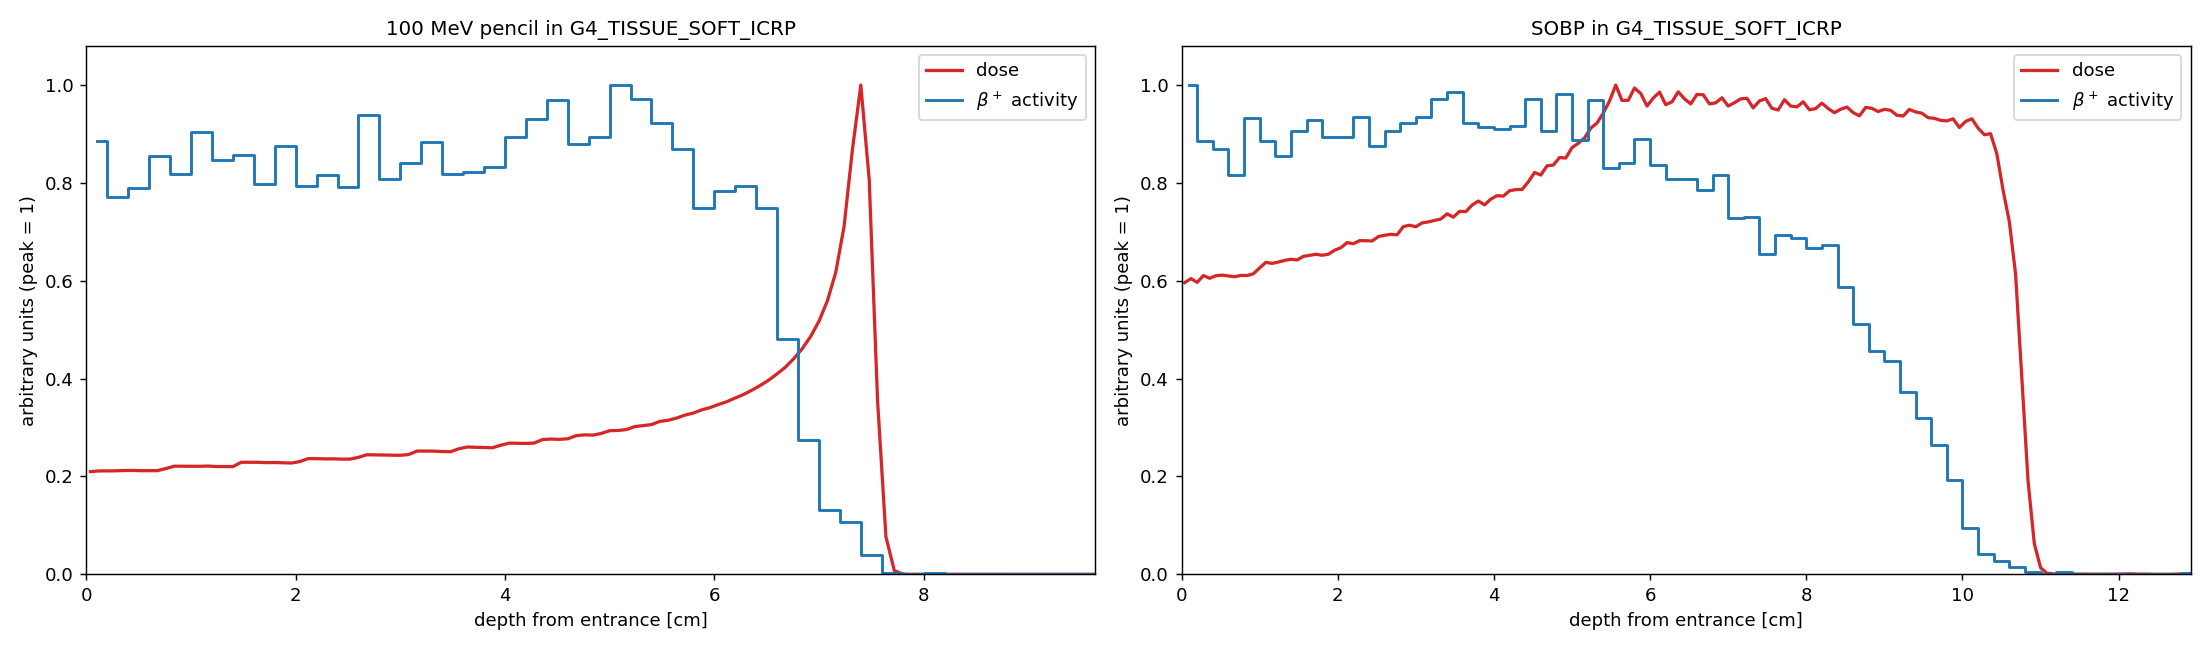
\includegraphics[width=\linewidth]{dose_activity.png}
\caption{Dose (red) and total $\bplus$ activity (blue), in arbitrary units (each
curve normalised to its own peak), for two beams in the same soft-tissue cylinder.
\emph{Left:} a \SI{100}{MeV} pencil --- a single Bragg peak. \emph{Right:} a
spread-out Bragg peak (SOBP), several energies combined into a flat dose plateau
across a target at \SIrange{5.5}{10.5}{cm} depth. In both cases the $\bplus$
activity is roughly flat along the proton track and falls to zero just before the
distal dose edge; that fall-off, $A(x)\to 0$, marks the beam's distal reach.}
\label{fig:source}
\end{figure}

The left panel of Figure~\ref{fig:source} shows a pencil beam depositing a dose $D$ in biological tissue. The sharp Bragg peak defines the maximum of dose deposition. The figure also shows the total $\bplus$ activity, which would correspond to an ideal PET measurement starting acquisition immediately after the beam stops.

The activity curve and the dose behave differently. As the proton beam propagates through the tissue, before the target region (and the Bragg peak), the dose is low and slowly rising, and the $\bplus$ activity is relatively flat. At the Bragg peak the beam quickly loses energy, quenching the nuclear reactions, so the $\bplus$ activity drops just where the Bragg ionisation rises and reaches zero in the trailing edge of the peak. Formally, if $A(x)$ is the activity along the beam line, the distal reach of the beam is estimated by the point $x'$ at which $A(x')=0$.

The right panel of Figure~\ref{fig:source} shows the same comparison for a spread-out Bragg peak --- the field used in treatment, where several proton energies combine to deliver a flat dose plateau across the target volume. The same reasoning holds: the $\bplus$ activity is roughly flat across the plateau and falls to zero just past its distal edge, so $A(x) \rightarrow 0$ marks the distal edge of the target volume.

Several physical effects complicate this simple picture. A PET scanner does not directly measure activity, only pairs of gammas; the activity must be reconstructed from the data, a non-trivial task. A scanner records only a fraction of the produced gamma pairs, once geometrical and detector efficiency are folded in. And the $\bplus$ reach --- the distance a positron travels before annihilation --- introduces a genuine physical uncertainty in the determination of the distal edge of the beam.

The example just described is also idealised: a cylinder filled with biological tissue. In practice the proton beam propagates through a heterogeneous medium, which complicates the picture further, and motivates the field design of the next section.

\section{Spread-out Bragg peak: field design}
\label{sec:sobp}

The standard field is a spread-out Bragg peak: a superposition of mono-energetic
beams whose ranges span the target depth and whose fluence weights flatten the
dose across it. The depth component of such a field can be built analytically, as
follows.

\subsection{Mono-energetic proton beam}
\label{sec:pristine}

A mono-energetic proton of energy $E$ stops at a well-defined depth, its
\textbf{range} $R$. To good approximation the two are related by the
Bortfeld power law~\cite{bortfeld1996},
\begin{equation}
R(E) = \alpha\,E^{\,p},
\label{eq:range}
\end{equation}
with, in water, $\alpha=\SI{2.2e-3}{cm\,MeV^{-p}}$ and $p=1.77$. For another
homogeneous material the range scales by the (mass) stopping-power ratio,
which to first order is the inverse mass-density ratio,
$R_{\mathrm{mat}}\simeq R_{\mathrm{water}}/\rho_{\mathrm{rel}}$
($\rho_{\mathrm{rel}}\approx1.04$ for brain). The energy needed to reach a depth
$R$ is the inverse of Eq.~\eqref{eq:range}, $E(R)=(R/\alpha)^{1/p}$.

Equation~\eqref{eq:range} fixes the \emph{layer energies}. A further consequence is
useful: a proton that has travelled to depth $z<R$ has residual range $R-z$ and
residual energy $\propto (R-z)^{1/p}$, so its mass stopping power (dose per unit
length) scales as
\begin{equation}
S(z;R)\ \propto\ \frac{\mathrm dE}{\mathrm dz}\ \propto\ (R-z)^{\,1/p-1}.
\label{eq:stop}
\end{equation}
This is the only feature of the peak shape the weight derivation needs.

\subsection{SOBP as a weighted superposition}
\label{sec:super}

A SOBP superimposes $N$ mono-energetic Bragg peaks at ranges $R_i$ spanning the
target depth,
\begin{equation}
R_i = \Rp + \frac{i}{N-1}\,(\Rd-\Rp),\qquad i=0,\dots,N-1,
\end{equation}
($R_0=\Rp$ proximal, $R_{N-1}=\Rd$ distal), with relative fluence weights
$w_i\ge0$. The total depth--dose is their superposition,
\begin{equation}
D_{\mathrm{SOBP}}(z)=\sum_{i\,:\,R_i\ge z} w_i\,S(z;R_i).
\label{eq:super}
\end{equation}

\subsection{Analytic flattening weights}
\label{sec:weights}

The target is a flat plateau, $D_{\mathrm{SOBP}}(z)=\text{const}$ for
$z\in[\Rp,\Rd]$. Treating the range as continuous with fluence density $\Phi(R)$,
Eq.~\eqref{eq:super} with \eqref{eq:stop} becomes the Abel-type integral
\begin{equation}
D(z)=\int_z^{\Rd}\Phi(R)\,(R-z)^{1/p-1}\,\mathrm dR =\text{const}.
\end{equation}
This is an Abel (right-sided fractional) integral equation of order $a=1/p$;
inverting it for a constant left-hand side gives
\begin{equation}
\boxed{\;\Phi(R)\ \propto\ (\Rd-R)^{-1/p}\;}\qquad R\in[\Rp,\Rd],
\label{eq:phi}
\end{equation}
The exact inversion also contains a point fluence at the proximal edge $R=\Rp$
that squares off the proximal corner; the discrete design omits it, and the
corner rounds over one layer spacing, within the plateau tolerance. Since
$-1/p\approx-0.565<0$, the weight rises towards the
\emph{distal} peak (which no deeper peak reinforces) and diverges integrably at
$R=\Rd$. Integrating Eq.~\eqref{eq:phi} over each range bin
$[R_i-\tfrac{\Delta}{2},\,R_i+\tfrac{\Delta}{2}]$ (with $\Delta=(\Rd-\Rp)/(N-1)$)
gives the finite discrete weights
\begin{equation}
\tilde w_i\ \propto\ (\Rd-R_i+\tfrac{\Delta}{2})^{1-1/p}-(\Rd-R_i-\tfrac{\Delta}{2})^{1-1/p},
\label{eq:wi}
\end{equation}
with both arguments clipped at zero so the distal bin stays finite (no peaks lie
beyond $\Rd$).

\subsection{Attenuation correction}
\label{sec:atten}

Equation~\eqref{eq:wi} flattens the \emph{ideal} superposition, but the
\emph{delivered} field droops from proximal to distal: protons are lost on the
way in (mainly to nuclear reactions), so deeper layers arrive depleted. To
compensate, each layer is boosted by an exponential in its range,
\begin{equation}
w_i\ \propto\ \tilde w_i\,e^{\mu R_i},
\label{eq:atten}
\end{equation}
with $\mu$ [\si{cm^{-1}}] a single effective coefficient tuned so the
\emph{simulated} plateau is flat (the standard value is
$\mu=\SI{0.025}{cm^{-1}}$). The weights are then normalised, $\sum_i w_i=1$. The
matching attenuation factor $e^{-\mu z}$ appears in the analytic depth--dose used
for the sanity plot.

\subsection{Heterogeneous media: water-equivalent path length}
\label{sec:wepl}

The scaling of Section~\ref{sec:pristine} used a single density ratio
$\rho_{\mathrm{rel}}$, correct for a \emph{homogeneous} phantom. The general case
calls for a heterogeneous medium. A head, for example, presents the beam with soft
tissue, a bone skull shell, brain, then bone again. Cortical bone stops protons far
more strongly than its density alone suggests, so a water- or brain-tuned layer set
lands the whole stack proximal. The remedy, standard in treatment planning, is to
design in \textbf{water-equivalent path length} (WEPL).

\subsubsection{Relative stopping power}
The \textbf{relative stopping power} (RSP) of a material is its proton mass
stopping power divided by water's at the same energy. From the Bethe formula,
\begin{equation}
\mathrm{RSP}(E)=\eta_{\mathrm{rel}}\,
\frac{\ln\!\big(2 m_e c^2\beta^2\gamma^2/I_{\mathrm{mat}}\big)-\beta^2}
{\ln\!\big(2 m_e c^2\beta^2\gamma^2/I_{\mathrm{water}}\big)-\beta^2},
\label{eq:rsp}
\end{equation}
where
$\eta_{\mathrm{rel}}=\dfrac{\rho_{\mathrm{mat}}}{\rho_{\mathrm{water}}}
\dfrac{\sum_k w_k Z_k/A_k}{\left.\sum_k w_k Z_k/A_k\right|_{\mathrm{water}}}$
is the relative electron density (from the elemental mass fractions $w_k$ and
their $Z_k/A_k$) and $I$ is the mean excitation energy. RSP depends
only weakly on energy, so it is enough to evaluate Eq.~\eqref{eq:rsp} at a representative
\SI{150}{MeV}; this gives $\mathrm{RSP}\approx1.03$ (soft tissue), $1.04$ (brain),
$1.71$ (cortical bone). Equation~\eqref{eq:rsp} is the principled form of the
$1/\rho_{\mathrm{rel}}$ scaling of Sec.~\ref{sec:pristine}, the analytic analogue
of a treatment-planning system's Hounsfield-unit$\to$RSP calibration.

\subsubsection{Water-equivalent path length}
The \textbf{WEPL} to a depth $d$ along the central axis is the thickness of water
that would slow the proton equally: the geometric path reweighted by RSP,
\begin{equation}
\mathrm{WEPL}(d)=\int_0^{d}\mathrm{RSP}\big(\mathrm{material}(z)\big)\,\mathrm dz
\;=\;\sum_k t_k\,\mathrm{RSP}_k ,
\label{eq:wepl}
\end{equation}
the sum running over the materials the axis crosses ($t_k$ their thicknesses). In
WEPL the Bragg curve is \emph{universal}: a proton of water range $R$ stops where
the accumulated WEPL equals $R$, whatever it traversed. For the standard head axis
to the proximal target ($d=\SI{55}{mm}$: ${\sim}\SI{4}{mm}$ scalp, \SI{8}{mm}
bone, \SI{43}{mm} brain),
\[
\mathrm{WEPL}=4(1.03)+8(1.71)+43(1.04)\approx\SI{62}{mm},
\]
i.e.\ the bone pushes the radiological depth ${\sim}\SI{7}{mm}$ beyond the
geometric one; the distal target maps similarly to ${\sim}\SI{114}{mm}$.

\subsubsection{Designing through the head}
The SOBP is then built exactly as before, but in WEPL:
\begin{enumerate}[nosep]
\item Ray-trace Eq.~\eqref{eq:wepl} along the axis to map the \emph{geometric}
target window $[\Rp,\Rd]$ to its \emph{water-equivalent} window
$[\mathrm{WEPL}(\Rp),\mathrm{WEPL}(\Rd)]$ (the implementation accumulates
Eq.~\eqref{eq:wepl} in \SI{0.05}{mm} steps along the central axis, from the
entrance face, with air contributing zero).
\item Run the layer design of Secs.~\ref{sec:weights}--\ref{sec:atten} on that
window with $\rho_{\mathrm{rel}}=1$ (the medium conversion now lives in the WEPL
map, not in a scalar). The Abel weights, Eq.~\eqref{eq:wi}, are \textbf{unchanged}:
in WEPL space the plateau is flat by the same construction, and since
$\mathrm{dose}/\mathrm d(\text{geom})=\big[\mathrm{dose}/\mathrm d(\mathrm{WEPL})\big]
\times\mathrm{RSP}$ with RSP nearly constant across the brain target, the geometric
plateau is flat where it matters.
\end{enumerate}
Because both the medium (through WEPL) and the target window enter the design,
different phantoms require different layer tables: the field is specific to the
phantom, not universal.

\begin{figure}[htbp]
\centering
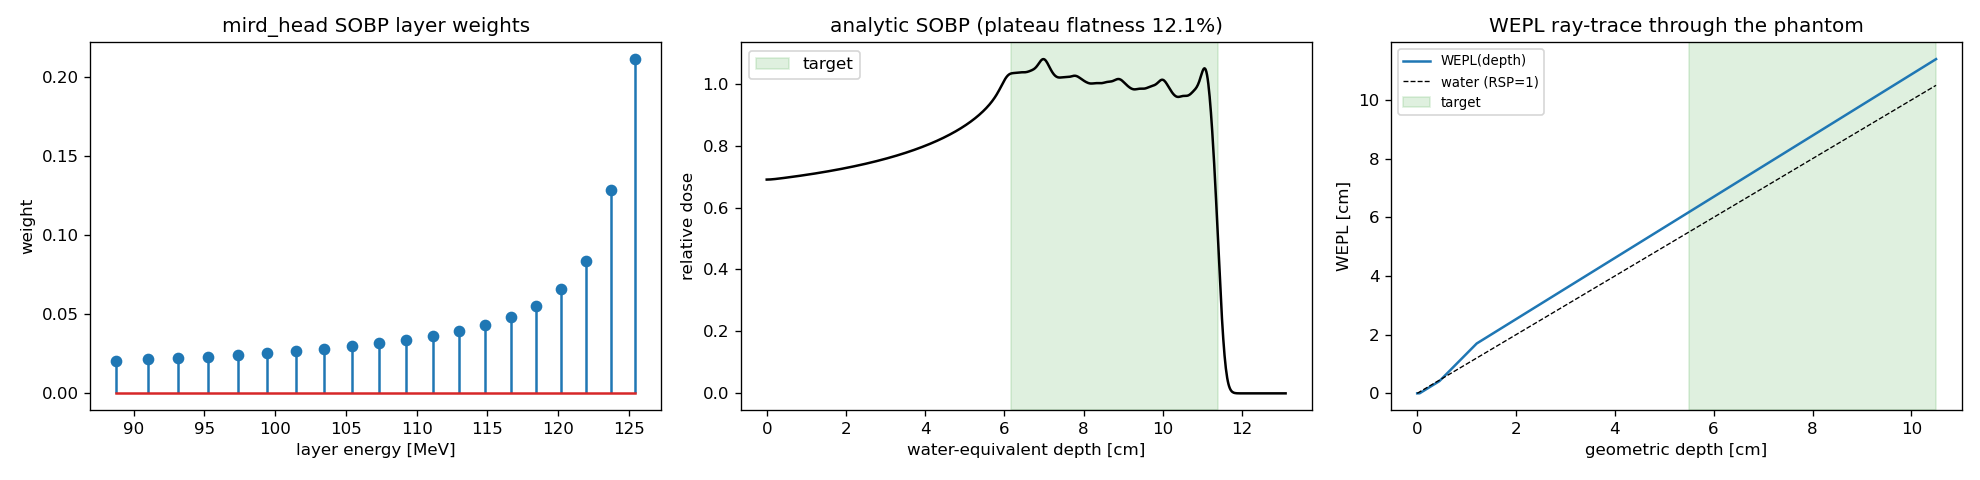
\includegraphics[width=\linewidth]{wepl_design.png}
\caption{WEPL field design for the MIRD head.
\textbf{Left:} the Abel flattening weights (Eq.~\eqref{eq:wi}), heaviest on the
distal layer. \textbf{Centre:} the resulting analytic SOBP, flat across the target
in water-equivalent depth. \textbf{Right:} the WEPL ray-trace along the central
axis (Eq.~\eqref{eq:wepl}) --- the curve rises above the water diagonal, with the
kink in the first ${\sim}\SI{1.2}{cm}$ where the beam crosses scalp then skull
bone, so the geometric target window $[\SI{5.5}{},\SI{10.5}{}]\,\si{cm}$ maps to
$[\SI{6.2}{},\SI{11.4}{}]\,\si{cm}$ WEPL. This shift is the bone offset the design
absorbs.}
\label{fig:wepl}
\end{figure}

A residual limit remains. The ray-trace is one-dimensional, along the central
axis; off-axis rays of the lateral field cross slightly different skull thickness,
and WEPL corrects the mean range shift but not the extra straggling and
multiple-scattering broadening at the bone interface. Plateau uniformity over the
target volume, rather than along the axis alone, is therefore the physical test of
the design.

\section{From equations to code}
\label{sec:eq-code}

Each derivation of this note is implemented by one function in the repository;
the table maps them.
\begin{center}
\begin{tabular}{@{}lll@{}}
\toprule
equation & implements & function \\
\midrule
\eqref{eq:nmeas} & three-factor measured decays $N_j$ & \texttt{decay\_sampling/budget.py:survival} \\
\eqref{eq:pj} & dose normalisation $P_j(D)$ & \texttt{decay\_sampling/budget.py} \\
\eqref{eq:pool} & pool floor on the recovered range & \texttt{analysis\_transport/distal\_pool.py} \\
\eqref{eq:range} & Bortfeld range--energy & \texttt{field\_design/sobp.py:energy\_for\_range} \\
\eqref{eq:wi}, \eqref{eq:atten} & layer weights $+$ attenuation boost & \texttt{field\_design/sobp.py:design} \\
\eqref{eq:rsp} & relative stopping power & \texttt{common/phantom\_material.py:relative\_stopping\_power} \\
\eqref{eq:wepl} & WEPL ray-trace & \texttt{field\_design/sobp.py:wepl\_curve} \\
\bottomrule
\end{tabular}
\end{center}
The activity curves of Fig.~\ref{fig:activity} are drawn by
\texttt{decay\_sampling/activity\_plot.py} and the dose--activity overlay of
Fig.~\ref{fig:source} by \texttt{analysis\_transport/plot\_dose\_activity.py},
both from simulated runs.

\bibliographystyle{unsrt}
\bibliography{biblio}

\end{document}
